\subsection{Starting Fresh}
\label{sec:loadSourceMeta}
\begin{itemize}

\item[$\blacktriangleright$] Press the \texttt{new} button on the Eclipse toolbar and navigate to ``Examples/eMoflon Handbook Examples/''
(Fig.~\ref{eclipse:downPartIV}). There are two cheat packages for eMolfon's two specification types. They each contain the full \texttt{LeitnersLearningBox}
metamodel, as well as the methods implemented as SDMs, and an instance of your model. For a brief discussion on the differences between the types, refer to Part
I, Section I.

\begin{figure}[htbp]
\begin{center}
  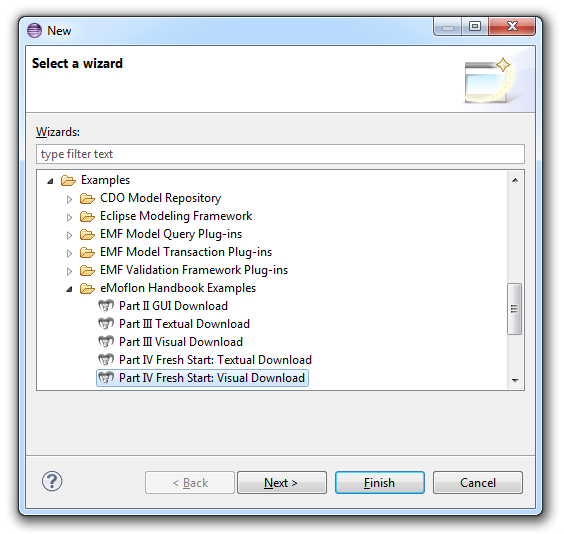
\includegraphics[width=0.7\textwidth]{eclipse_part4FreshWizardDownload}
  \caption{Download your preferred metamodel specification type}
  \label{eclipse:downPartIV}
\end{center}
\end{figure}

\item[$\blacktriangleright$] After loading, if your package explorer does not resemble ours in Fig.~\ref{eclipse:workingSets} with at least two
distinct nodes, select the small, downward facing arrow in the corner of the module window. Choose ``Working Sets/Top Level Elements.'' To review how these
nodes are used to structure the workspace in Eclipse, check out Part I, Section 4.

\vspace{0.5cm}

% Forced placement so it would co-operate
\begin{figure}[htbp]
	\centering
  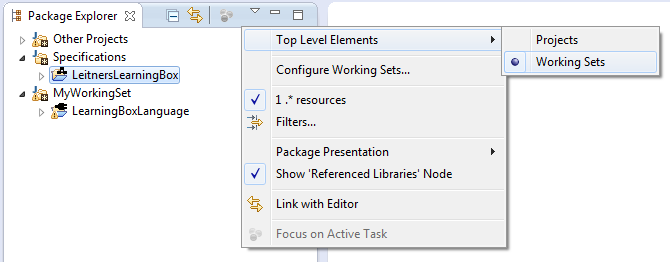
\includegraphics[width=0.9\textwidth]{eclipse_workingSets}
	\caption{Setting your Package Explorer}
	\label{eclipse:workingSets}
\end{figure}

\item[$\blacktriangleright$] Fantastic -- you now have the first piece of your tranformation triple ready to go!

\end{itemize}